\textsc{Nenwin} is able to simulate other computational mechanisms\footnote{
or, equivalently, other computational mechanisms can be reduced to \textsc{Nenwin}. 
'Reduction' causes less ambiguity than 'simulate', as \textsc{Nenwin} is implemented via an simulation itself.}. 
In particular, this section will demonstrate that \textsc{Nenwin} is able to simulate all required components to implement a CPU. 
A CPU is an implementation of the RAM-model, which is equivalent to a Turing machine \cite{RAM_cook_reckhow}.

This section will demonstrate that \textsc{Nenwin} is able to simulate the following components, when using Marbles as data-carrying signals:
\begin{itemize}
    \item A Boolean NAND-gate with interfaces that use Marbles to transmit and receive information. Note that all binary logical functions such as OR, AND, NOT, NOR, etc. can be implemented from compositions of NAND-gates.
    \item A single-bit register that can store a state 0 or 1. Note that an arbitrary large composition of bit registers can store an arbitrary large amount of data.
    \item A clock that creates periodically a signal.
    \item A \textit{divider}: a component that upon intercepting one Marble, creates multiple Marbles with velocities in different directions. In the context of wires and electricity such devices are not needed, but in the context of discrete Marbles it is required.
\end{itemize}

These reductions demonstrate that \textsc{Nenwin} is theoretically powerful enough 
to solve the same problems as the simulated components.  However, they are not necessary of any practical use otherwise, as it is slower than directly implementing/simulating the other computational mechanisms they simulate.
These reductions use very artificial hand-made (in contrast to automatically optimized) architectures that 
do not exploit the dynamic nature of \nenwin. This generally allows simpler proofs. 
For example, immovable Nodes result in much less complex proofs than with moving Nodes. 

\nenwin is by default non-terminating, 
but it can simulate terminating algorithms when a consistent rule is used to determine the moment when output is read.
One natural such rule is to read output when all Marble's have disappeared, 
as the output will not change any more after this point.

Consider a variant of Newton's gravity function, called the 'threshold gravity', that rounds the force to 0 when the radius is sufficiently large:
\begin{equation}
    threshold\_gravity(p_1, p_2, \theta) = \begin{cases}
        \vec{0} & \text{ if } \doublenorm{p_1.pos - p_2.pos} > \theta \\
        \frac{p_1.m \cdot p_2.m}{\doublenorm{p_1.pos - p_2.pos}^2} & \text{otherwise}
        \end{cases} \label{eq:tresholdgrav}
\end{equation}

Unless stated otherwise, this threshold-gravity force function \eqref{eq:tresholdgrav} will be used as attraction function by all particles in this section.

All figures will use the same convention of drawing particles. A legend of this convention is shown below in Fig. \ref{fig:legend}.

\begin{figure}[h]
	\centering
	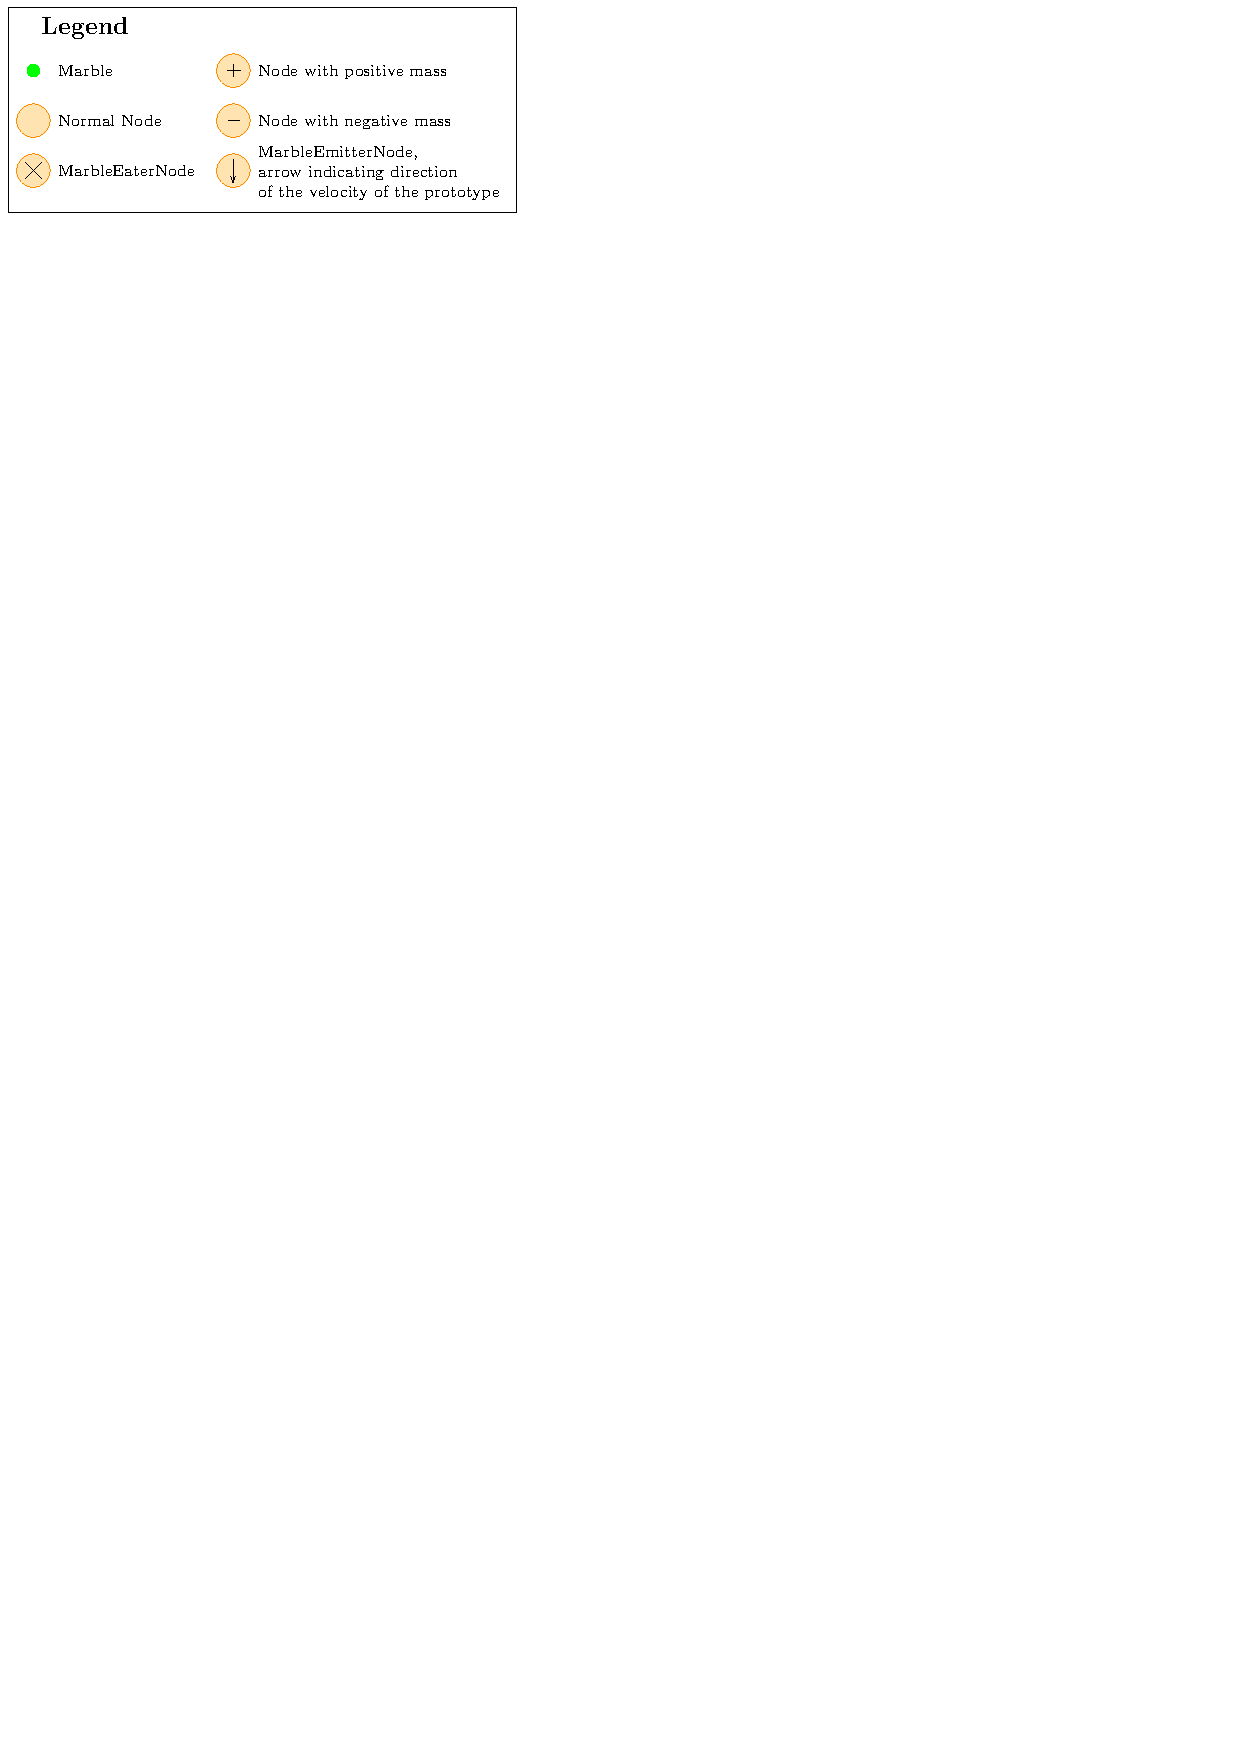
\includegraphics[scale=1.1]{figures/legend.pdf}
	\caption{Legend of the figures describing \nenwin architectures. 
		Marbles are depicted as green dots, and nodes as orange disks.
		MarbleEaterNodes and MarbleEmitterNodes have a special annotation, namely an '$\times$' for MarbleEaterNodes, 
		and an arrow for MarbleEmitterNodes. 
		This arrow indicates the direction of initial the velocity of emitted Marbles 
		(or, equivalently, the direction of the velocity of the prototype Marble).
		When relevant for the context, normal Nodes may also be annotated with the polarity of their mass.}
	\label{fig:legend}
\end{figure}

\subsection{NAND-gate}
The \textsc{Nenwin}-scheme is able to simulate a logical NAND-gate.
As a NAND-gate is a Boolean function with only two Boolean input values, there are only 4 different input combinations that need to be handled correctly. Below it is shown how \textsc{Nenwin} can directly simulate a NAND-gate with inputs and output to the \textsc{Nenwin} program itself, and how a NAND-gate can be embedded in a larger circuit within a \textsc{Nenwin}-architecture. 

Let $\mathcal{M}$ denote the set of all possible marbles and $\mathcal{N}$ the set of all possible nodes. 
\begin{lemma}[NAND-gate]
There exists an input placer mapping a vector of two Boolean variables to a set of Marbles $f:\{0, 1\}^2 \rightarrow\mathcal{M}^2$,
a \textsc{Nenwin} architecture of only nodes $A \subseteq \N$, and a function to map the \nenwin output to a Boolean output $g:\mathbb{N}^2 \rightarrow \{\false, \true\}$,\\
such that for two Boolean variables $b_1, b_2 \in \{\false, \true\}$, $g(\vec{y}) = \neg (b_1 \land b_2)$, where $\vec{y}$ is the output harvested from architecture $A$ with input $\{f(b_1), f(b_2)\}$ after all marbles were removes from the network.
\label{lemmma:nand_simple}
\end{lemma}
\begin{proof}

    For all particles we will use \texttt{node\_stiffness} = 0, 
    \texttt{marble\_stiffness} = 1, \texttt{node\_attraction}=0 and \texttt{marble\_attraction}=1.

    Define 
    \begin{equation}
        f(b) = \begin{cases}
            &\texttt{Marble}(pos=[10, 0], vel=\vec{0}, acc=\vec{0}, mass=+10, datum=\textsc{True}) \quad \text{if $b = \textsc{True}$} \\
            &\texttt{Marble}(pos=[10, 0], vel=\vec{0}, acc=\vec{0}, mass=-10, datum=\textsc{False}) \quad \text{if $b = \textsc{False}$}
        \end{cases}
    \end{equation}
    
    Let
    \begin{align}
        A = &[ \nonumber \\
        & \texttt{MarbleEaterNode}(pos=[0, 0], vel=\vec{0}, acc=\vec{0}, mass=+10, radius=5) \nonumber \\
        & \texttt{MarbleEaterNode}(pos=[20, 0], vel=\vec{0}, acc=\vec{0}, mass=-10, radius=5) \nonumber \\
        &]
    \end{align}

    Define 
    \begin{equation}
        g(\vec{y}) = \begin{cases}
                    \false &\text{if } y[0] = 2 \\
                    \true &\text{if } y[0] \in \{0, 1\}
        \end{cases}
    \end{equation}
    
    Note that the Marbles are placed in the middle of the line-segment between the two Nodes, 
    and that positive masses attract positive masses and repel negative masses, and vice versa. 
    Hence each of the two Marbles will be accelerated in a straight line to the Node with the same polarity of mass as itself, 
    and will be eaten by it.
    
    Now if the input is $(\true, \true)$, both Marbles will have a positive mass of 10, and both will be attracted to the left Node (at $pos[0] = 0$ with mass +10). This way both will be absorbed by the first Node, and the output will read $g(\begin{bmatrix}2\\0\end{bmatrix}) = \false$ as expected.
    
    If the input equals $(\true, \false)$, $(\false, \true)$, $(\false, \false)$, then at least one Marble will be attracted and eaten by the right node (at $pos[0] = 20$ with mass -10), and since there are only 2 Marbles, no more than one Marble will be eaten by the left Node, and the output is $g(\begin{bmatrix}1\\1\end{bmatrix})$ or $g(\begin{bmatrix}0\\2\end{bmatrix})$, either of which will evaluate to $\true$ as expected.
\end{proof}
See Fig. \ref{fig:nand_simple} for a visualization of the proof.

\begin{figure}[h]
	\centering
	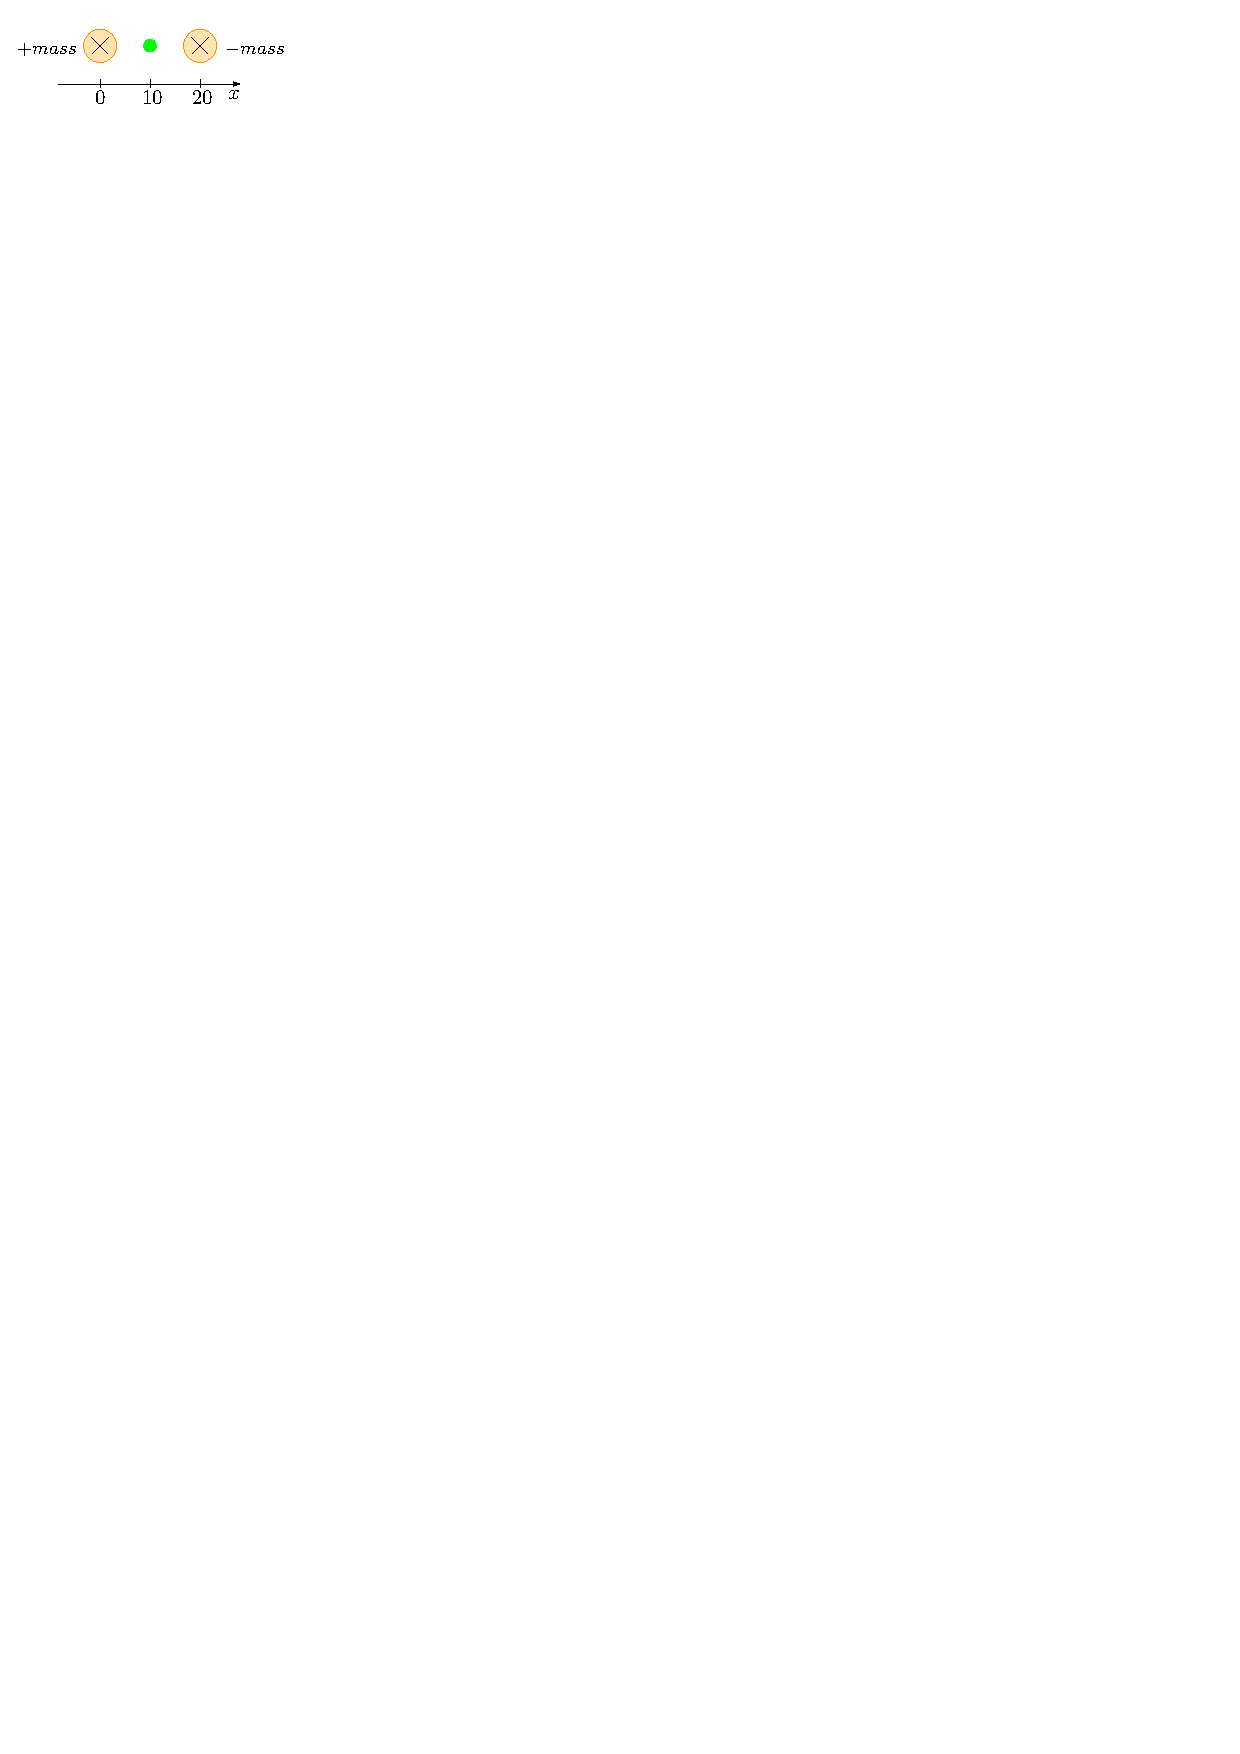
\includegraphics[scale=1.5]{figures/nand_simple.pdf}
	\caption{Construction of a NAND-gate in \nenwin as used by the proof of Lemma \ref{lemmma:nand_simple}. The left Node has a positive mass, and the right Node a negative mass. Note that only one dimension (the $x$-axis) is used, and that both Marbles are placed by the input placer on exactly the same position (at $x = 10$).}
	\label{fig:nand_simple}
\end{figure}
\clearpage

The above lemma does not show how a NAND-gate can be implemented as part of a larger circuit. To achieve this, all that is needed is a NAND-gate that has a finite region of $\mathbb{R}^3$ in which it attracts particles (so that the rest of the circuit can be implemented safely outside this region), and interfaces to the other parts of the circuit. 

In this series of proofs, such interfaces are represented by MarbleEmitterNodes (and MarbleEaterNodes for output interfaces, which can easily be replaced by MarbleEmitterNodes). The main advantage of user MarbleEmitterNodes is that it gives more control over how the input signal is send into a circuit module (esp. in terms of velocity and direction), in comparison to allowing external Marbles to directly enter the module.

The next lemma will show that is possible to extend the NAND-gate with interfaces to an external circuit. It uses a different encoding for \textsc{True} and \textsc{false}: the presence and absence respectively of positively massed Marbles (with a mass of $\alpha$). Note that the direction and velocity if the Marbles emitted by the output MarbleEmitterNodes can be configured. Furthermore, the NAND-gate requires external 'power' to operate: this can be compared to electronic NAND-gates requiring an operating voltage that is separate from the signal. This 'power' needs to be the same for each input, and hence does not externally provide information about the input.

\begin{lemma}
    Given positive constants $\alpha \in \mathbb{R}$, a finite cuboid $C \subseteq \mathbb{R}^3$, a finite set of particles in a plane $P \subset C$, and an external Marble $m_{power}$ with a mass of $-\alpha$, \nenwin is able to simulate a NAND-gate using two MarbleEmitterNodes at the boundaries of $C$ as interfaces, such that the particles in $C$ influences no particles beyond $C$ except for creating output Marbles, when \textsc{True} and \textsc{False} are encoded as presence and absence respectively of positively massed Marbles with a mass of $\alpha$. The NAND-gate creates an output after a finite amount of time, and at this time the NAND-gate returns to a state in which it will produce the same output for the same input.
    \label{lemma:nand_with_iface}
\end{lemma}
\begin{proof}
    The lemma will be proven using a construction. This construction is the concatenation of an AND-gate and a NOT-gate.
    
    Define the following particles in the 'AND' part (also see Fig. \ref{fig:nand_with_iface}). All EmitterNodes and EaterNodes will be initialized with a \texttt{stored\_mass} of 0 and no attraction (which is achieved by setting their Marble-attraction and Node-attraction values to 0 \footnote{Alternatively, the state of no attraction could be achieved by giving the Nodes a mass of 0. This distinction is not relevant for the proof.}):
    \begin{itemize}
        \item A signal-emitter: a MarbleEmitterNode in $P$ with a position and radius such that the border of the radius intersects the border of $C$ in one point $p$. This Node functions as the input interface of the NAND-gate, as zero up to two external Marbles serving as input can be consumed by the signal-emitter at point $p$. It has a positive emitting-delay of $\delta \in \mathbb{R}$.
        
        \item A signal-Marble: the Marble that can be emitted by the signal-emitter. It has of mass $\alpha$ with a positive velocity in the direction of the vector from the signal-emitter towards the center of $P$ (this direction will for convenience by called $e_y$ from now, using the axes as in Fig. \ref{lemma:nand_with_iface} we have $up = \begin{bmatrix}x\\ y\\ z\end{bmatrix} = \begin{bmatrix}0\\ 1\\ 0\end{bmatrix}$). The velocity has a magnitude of $v$. It has a Marble-stiffness of 0 and a Marble-attraction of 1.
        
        \item A signal-accumulator: a MarbleEmitterNode in $P$ placed a distance $d_{AND} \in \mathbb{R}^{+}$ from the signal-emitter in the direction $e_y$. $d_{AND}$ is chosen such that the point that is positioned at a positive $d_{NOT}$ in the direction $e_y$ from the signal-accumulator is in $C$. This Node acts as the logic in the AND-part: it emits Marbles with a mass of $2\alpha$, hence it can only emit if the signal-emitter has emitted two Marbles, which only occurs if the signal-emitter has two inputs of value \textsc{True}.
        
        \item A resetter-emitter: a MarbleEmitterNode positioned in $P$, such that it it a distance of $\frac{1}{2}d_{AND} + \psi$ (for a small constant $\psi > 0$) from the center $k$ of the line-segment between the signal-emitter and the signal-accumulator, at a an angle in $(0 \deg, 90 \deg)$ with the line-segment between the signal-accumulator and $k$. It has a radius such that the border of the radius intersects the border of $C$. Note that the signal-accumulator, the signal-emitter and the resetter-emitter are all a distance $\frac{1}{2}d_{AND}$ from $k$. It has an emitting-delay of $2 \delta$.
        
        \item A resetter-Marble that can be emitter by the resetter-emitter, which has a mass of $-\alpha$, a velocity of magnitude $v$ and a velocity-direction towards $k$ from the point where it is emitter. It has a Marble-stiffness of 0 and a Marble-attraction of 1. Since it is directed towards $k$ with the same magnitude of velocity as the signal-Marble, these two Marbles will arrive at $k$ after the same time.
        
        \item An inhibitor-Marble that can be emitted by the signal-accumulator, and that has a velocity with a magnitude $v$ in the direction $e_y$. 
        \item Let $h$ be the point in $P$ that is a distance of $\frac{1}{2}d_{NOT}$ away from the signal-accumulator in the direction $e_y$. It has a Marble-stiffness of 0 and a Marble-attraction of 1.
        
        \item A not-emitter: a MarbleEmitterNode placed in $P$, with a delay of $2\delta + d_{AND} \cdot v$, emitting a Marble (the 'output-Marble') with a mass of $\alpha$ with a velocity with magnitude $v$ in the direction from the not-emitter towards $h$. The not-emitter is positioned such that the line segment between the not-emitter and $h$ has a length of $\frac{1}{2} d_{NOT} + \varepsilon$ (for a small constant $\varepsilon > 0$) and does not intersect any Node nor any line segment between a Node and $k$ or $h$ (see Fig. \ref{lemma:nand_with_iface}). Furthermore, the radius and the position are such that the border of the not-emitter intersects $C$.
        
        \item An output-Marble, as described above, with a Marble-stiffness of 0 and a Marble-attraction of 1.
        
        \item An output-emitter: a MarbleEmitterNode that acts as the output-interface. It is positioned in $P$ such that the line between the output-emitter and the not-emitter intersects $h$, but not any other line segment between a Node and $k$ or $h$, and such that the border of its radius intersects $C$.
        
        \item An accumulator-resetter-1, a MarbleEmitterNode positioned in $P$ such that if the resetter-Marble is repelled by the signal-emitter, its diverted path will lead to the signal-resetter-1. It has a nonnegative delay $\beta$.
        
        \item An accumulator-resetter-Marble, that has a positive velocity $u$ in the direction towards a point $i$ on the line segment between $h$ and the signal-accumulator. It has a mass of $-\alpha$, a Marble-stiffness of 0 and a Marble-attraction of 0. 
        
        \item An accumulator-resetter-2, also a MarbleEmitterNode positioned in $P$, on the ray that originates from the accumulator-resetter-1 and intersects $j$, at a greater distance from the first accumulator than $j$ has. It emits an identical Marble as the accumulator-resetter-Marble, but with a velocity directed towards the signal=accumulator. It has a nonnegative delay $\gamma$.
        
        \item Four garbage-collectors, MarbleEaterNodes all placed in $P$, that only serve to remove unneeded Marbles. One is placed at a distance $d_{NOT}$ in the direction $e_y$ from the signal-accumulator. Another one is placed at a location where the output-Marble will be recoiled towards (when it arrives at $h$ and the inhibitor Marble is at $h$ plus a distance $\varepsilon$ in direction $e_y$). The third one is placed on the ray that originates in the resetter-emitter and intersects $k$, at a greater distance from the resetter-emitter than $k$. The last garbage-collector is placed at a location where the accumulator-resetter-Marble will be recoiled towards from the point $j$, if it arrives at $j$ while the signal-Marble is a distance $\psi$ from $j$ in the direction $e_y$. 
    \end{itemize}
    
    The resetter-emitter and the not-emitter are the part of the gate that requires 'power', i.e. the NAND-gate only functions if these two MarbleEmitterNodes consume Marbles with an equal mass as the Marble they emit respectively, at the same moment as the input is consumed by the signal-emitter. Note that this 'power' can be supplied without disturbing the interior of $C$, as these MarbleEmitterNodes intersect the border of $C$, and the powering Marbles can have a Marble- and Node-attraction of 0.
    
    We now require that, if at some point in time $t_0$ (w.l.o.g. let $t_0 = 0$) the signal-emitter consumes 0, 1 or 2 Marbles with a mass of $\alpha$ (the presence of a Marble encodes the input value \textsc{True}, the absence the input value \textsc{False}), and the resetter-emitter and the not-emitter their required powering Marbles, then the NAND-gate should output a Marble with mass $\alpha$ outside of $C$ at a finite point in time $t_{end} > t_0$, unless two input Marbles are provided. We proceed by a case distinction on the number of input Marbles.
    
    \begin{enumerate}
        \item \textbf{0 input Marbles:} this corresponds to the input $(\textsc{False}, \textsc{False})$. In this case the signal-emitter will not emit any Marble. The resetter-emitter does emit a resetter-marble after a delay of $2\delta$, as it consumes a powering Marble with a mass of $-\alpha$ at the moment $t_0$ at which the empty input is 'given'. However, by construction of the NAND-gate, there is no particle or attraction force on the path of the resetter-Marble except for the garbage-collector, which will consume it. Similarly, the not-emitter will be powered and emit a Marble in the direction of the output-emitter, which will also arrive with its original velocity and direction unaffected at the output-emitter. Hence the \texttt{stored\_mass} of the output-emitter will reach the threshold to emit a Marble with mass $\alpha$ outside of $C$, which encodes the expected output \textsc{True}.
        
        \item \textbf{1 input Marble:} this corresponds to the input $(\textsc{True}, \textsc{False})$, or to the equivalent case $(\textsc{False}, \textsc{True})$. Hence the signal-emitter will emit a signal-Marble with a velocity in the direction of $e_y$. The signal-Marble's velocity will not be affected by the resetter-Marble, since the signal-marble has a Marble-stiffness of 1. There are no other attraction forces or particles along the line segment between the signal-emitter and the signal-accumulator, so the signal-Marble will be consumed by the signal-accumulator. This causes the signal-accumulator to obtain a \texttt{stored\_mass} of $\alpha$, which is not sufficient for it to emit a Marble.
        
        The resetter-emitter will also emit a resetter-Marble, which will arrive at the point $k$ when the signal-Marble is a distance $\psi$ in the direction $e_y$ from $k$ (this is, because both Marbles are emitted at the same time in a straight line to $k$ with the same velocity $k$, only the resetter-emitter needs to travel an additional distance $\psi$). If the the attraction threshold distance of the signal-Marble and the value of $\psi$ have been chosen correctly, then the resetter-Marble will be recoiled by the signal-Marble in a direction different than its original direction (as the signal-Marble is positioned in the direction of $e_y$ from the resetter-Marble, and the repelling force accelerated the resetter-Marble in the direction of the line from the signal-Marble to the resetter-Marble). So by construction the resetter-Marble will be redirected towards the accumulator-resetter-1 (the green arrow in Fig. \ref{fig:nand_with_iface}, which in turn will emit a Marble towards the accumulator-resetter-2, which in turn will emit a Marble towards the signal-accumulator. Since this Marble has an opposite mass as the signal-Marble that the signal-accumulator consumed, its \texttt{stored\_mass} will be reset to 0. It is possible that the negatively-massed Marble will be consumed before the signal-Marble instead, but clearly this leads to the same result \footnote{Alternatively, $\gamma$ (the delay of the accumulator-resetter-2) can be adjusted to ensure the signal-Marble will be consumed by the signal-accumulator first. This does not affect the resulting state of the particles of the NAND-gate.}. 
        
        The rest of the NAND-gate behaves identical as the case of \textit{0 input Marbles}, which leads to the correct output at the output-emitter.
        
        \item \textbf{2 input Marbles:} this corresponds to the input $(\textsc{True}, \textsc{True})$. In this case two signal-Marbles will be emitted, at $t = t_0 + \delta$ and at $t = t_0 + 2\delta$. As in the case of \textit{1 input Marble}, the first signal-Marble will be consumed by the signal-accumulator, and the resetter-Marble will be consumed by the accumulator-resetter-1. Now there exists a value for $\beta$ (the delay of the accumulator-resetter-1) such that there exists a small constant $\omega > 0$ such that the second signal-Marble is a distance $\omega$ in the direction $e_y$ from $j$ when the accumulator-resetter-Marble arrives at $j$. Similarly to the redirection of the resetter-Marble, this causes the accumulator-resetter-Marble to be redirected, which by construction sends the accumulator-resetter-Marble towards a garbage-collector (the yellow line in Fig. \ref{fig:nand_with_iface}).
        
        Hence the signal-accumulator will consume two Marbles each with a mass of $\alpha$ at $t = t_1 = t_0 + 2\delta +  d_{AND}\cdot v$ (where $d_{AND}\cdot v$ is the time needed for the second signal-Marble to travel from the signal-emitter to the signal-accumulator), but the accumulator-resetter-emitter-2 will not emit a Marble with negative mass, hence at $t_1$ the signal-accumulator will emit an inhibitor-Marble. This is also the time at which the not-emitter emits an output-Marble. 
        
        Similar to the first signal-Marble, the resetter-Marble and the point $k$, the output-Marble will arrive at the point $h$ when the inhibitor-Marble is a distance $\varepsilon$ in the direction $e_y$ from $h$. The inhibitor-Marble has a Marble-stiffness of 1, but the output-Marble has a Marble-stiffness of 0 and hence there exists a threshold distance for the inhibitor-Marble and a value for $\varepsilon$ such that the output-Marble will be shortly accelerated in the direction of the inhibitor-Marble. Then by construction, the output-Marble will be redirected to an garbage-collector (the purple line in Fig. \ref{fig:nand_with_iface} instead of the output-emitter. Also by construction, the inhibitor-Marble travels in a straight line from the signal-accumulator to a garbage-collector. Hence both particles will be consumed by garbage-collectors. Note that also the signal-accumulator now has a \texttt{stored\_mass} of 0, as the previously stored mass of $2\alpha$ has been depleted when emitting the inhibitor-Marble. 
        
        It can be concluded that, after the amount of time passed in which the NAND-gate produced output in the \textit{0 input Marbles} and \textit{1 input Marble} cases (which is the same time-span for both cases), no output will be produced, as required by the definition of a NAND-gate.
    \end{enumerate}
    Note that in all three cases, the NAND-gate eventually returned to the same state as before the input was given, except for the amount of Marbles eaten by the garbage-collectors. But the latter does not affect the behaviour of the NAND-gate, hence it will respond with the same outputs again given any of the three input cases above.
\end{proof}
\clearpage
\begin{figure}[h]
    \centering
    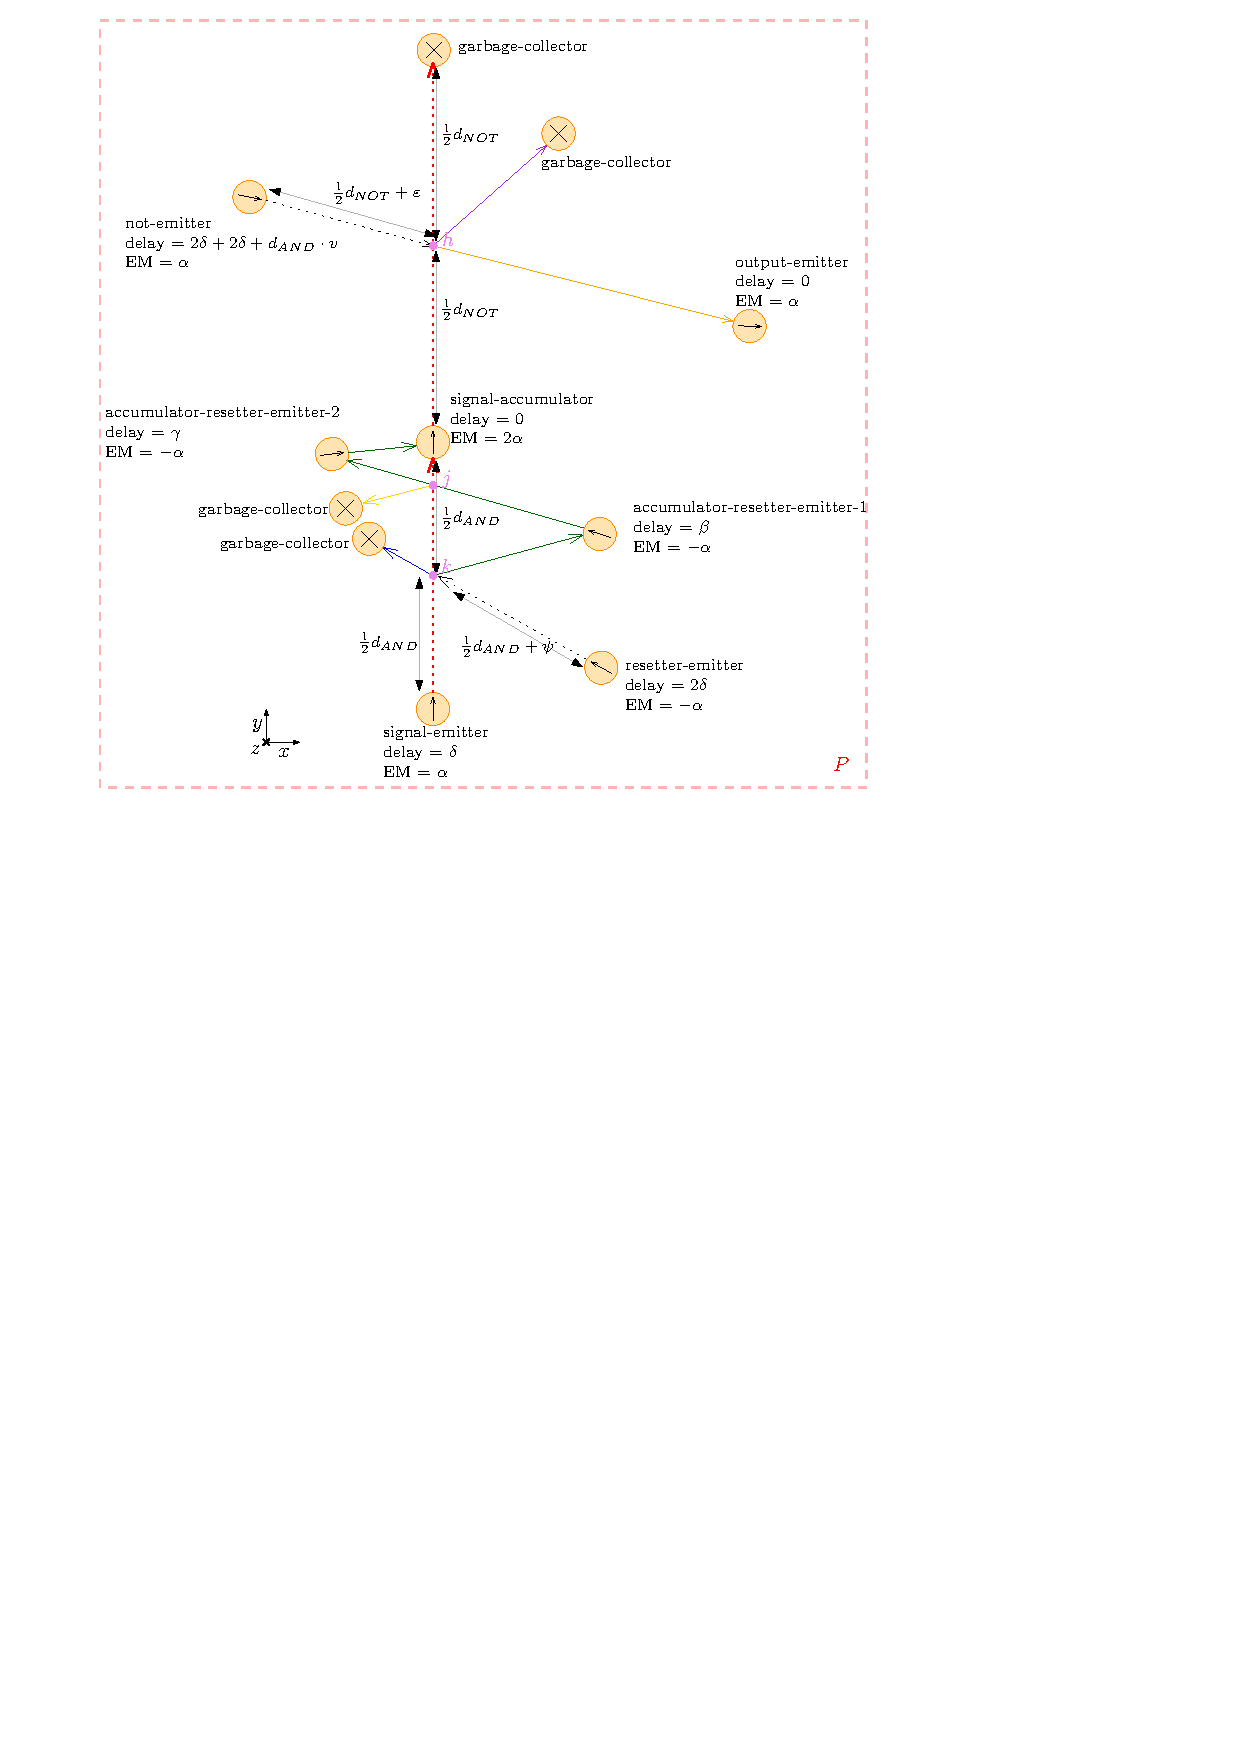
\includegraphics{figures/nand_with_interfaces_v6.pdf}
    \caption{Construction of a NAND-gate in \nenwin as used by the proof of Lemma \ref{lemma:nand_with_iface}. The axes of spatial coordinates $x$ and $y$ are parallel to the place $P$. For each MarbleEmitterNode, the emit-delay and the mass of the emitted marble (EM, 'Emitted Mass', for short) have been denoted. MarbleEmitterNodes are marked with an arrow that indicates the direction of the velocity of the Marble they can emit, and the MarbleEaterNodes (that is not also an EmitterNode) has been marked with a cross. Note that the distances between particles and the radii of the Nodes are not to scale.}
    \label{fig:nand_with_iface}
\end{figure}

\subsection{Tunnel}

Using the the threshold-gravity attraction function \eqref{eq:tresholdgrav}, is it possible to construct an architecture within a rectangular region that can 'steer' a Marble to any other side of the rectangle, and such that it does not interfere with the architecture outside the rectangle. This is proven in the lemma below. The result can be used as a black box in other proofs to 'tunnel' Marbles from one location to another.

\begin{lemma}[Tunnel] \label{lemma:tunnel}
    Let $R = [x_0, x_1] \times [y_0, y_1]$ be a rectangle in $\mathbb{R}^2$. Let $R$ be free of attraction forces from Nodes and Marbles not in $R$. Let $m$ be a Marble with nonzero mass that enters (not only intersects) $R$ via an edge $l$. Then for any point $p = (x_e, y_e)$ on the edges of $R$ that are not $l$, there exist finite numbers $\epsilon, \theta \in \mathbb{R}$ and a finite set of Nodes such that when placed in $R$, $m$ leaves $R$ via $p$.
\end{lemma}
\begin{proof}

    Without loss of generality, assume that $l$ is parallel to the $x$ axis, so all points on $l$ have $x$ coordinates in $[x_0, x_1]$, and the same $y$ coordinate $y_l$. Let $q = (x_q, y_l) \in l$ be the point where $m$ enters $R$.
    
    Let $h$ be the line segment between $q$ and the point $k$, where $k$ is the point where $m$ would have left $R$ if there were no other particles in $R$. Clearly $m$ would move through $R$ in a straight line segment if $R$ were free of other particles, as $R$ is free of forces from particles outside $R$, and hence $m$ would have 0 acceleration. Hence $k$ exists.
    
    If $x_0 < x_q < x_1$, then it is possible to place a Node $n$ with threshold gravity at threshold $\theta + \epsilon$, $\theta, \epsilon > 0$ at $(x_n + \theta, y_n) \in R$ such that the entire attraction field of $n$ is in $R$, $(x_n, y_n) \in h$, $(x_n, y_n) \neq q$ and $0 < \theta \in \mathbb{R}$. If we set $n.mass \leftarrow 0$, then $m$ will leave $R$ at $h$. 
    
    If we make the magnitude of $n.mass$ greater, and set $\sgn{n.mass} \leftarrow \sgn{m.mass}$, and hence the Node's attraction will change $m$'s course more towards the positive $x$ direction; by correct adjustment of $\theta$ and $n.mass$ can clearly adjust the strength of the acceleration and the duration, and hence can steer $m$ to leave $R$ at any point $(x_e, y_e)$ with $x_e > x$ on one of the non-$l$ edges of $R$.
    
    In a similar way, if we set $\sgn{n.mass} \leftarrow -1 \cdot \sgn{m.mass}$ and place $n$ at $(x_n - \theta, y_n) \in R$ instead, then we can steer $m$ to end up any point $(x_e, y_e)$ with $x_e < x$ on on of the non-$l$ edges of $R$.
    
    % If $x_q = x_0$ or $x_q = x_1$, then we can add a second node $n'$ at $(x_q + \theta', y_q)$ or $(x_q - \theta', y_q)$ respectively, with a threshold $\epsilon'$ much smaller than $\theta$. If we would not add a node $n$, then clearly $m$ would exit $R$ at a point $k = (x_k, y_k) \in R$ such that $x_0 < x_k < x_1$. Then let $h$ be the line segment between $q$ and $k$, and we can proceed the proof in a similar way as the case  $x_0 < x_q < x_1$.
    
    If $x_q = x_0$ or $x_q = x_1$, we can use the requirement that $m$ enters $R$, which implies that:
    \begin{enumerate}
        \item If $x_q = x_0$, then the $x$-component of $m.vel$ must be positive, otherwise $m$'s path would only intersect $R$ (move parallel to an edge or only pass the point $q$ no other point of $R$), but not enter it.
        \item If $x_q = x_1$, then the $x$-component of $m.vel$ must negative positive, by a similar argument.
    \end{enumerate}
    In both cases $k$ and $h$ will be well defined, and the construction as of the case $x_0 < x_q < x_1$ can be used.
\end{proof}

See \ref{fig:tunnel} for a visualization of the construction of the proof. 

A conceptually much simpler, but less efficient, method of implementing a 'tunnel' would be to use MarbleEmitterNodes and Marbles, both with 0 Node-attraction and Marble-attraction, in a region of the simulation where no external forces apply: here the Marbles can travel in straight lines between the MarbleEmitterNodes, which provides a method of controlling the movement of Marbles in a sufficiently simple way that it can be designed by hand. One major advantage of this method is that delays can be added to the MarbleEmitterNodes: this way it can be precisely regulated when a Marble will reach the end of the 'tunnel'. Also the velocity magnitude and direction of the resulting Marble emitted by the last MarbleEmitterNode can easily be adjusted.

\begin{figure}[h]
    \centering
    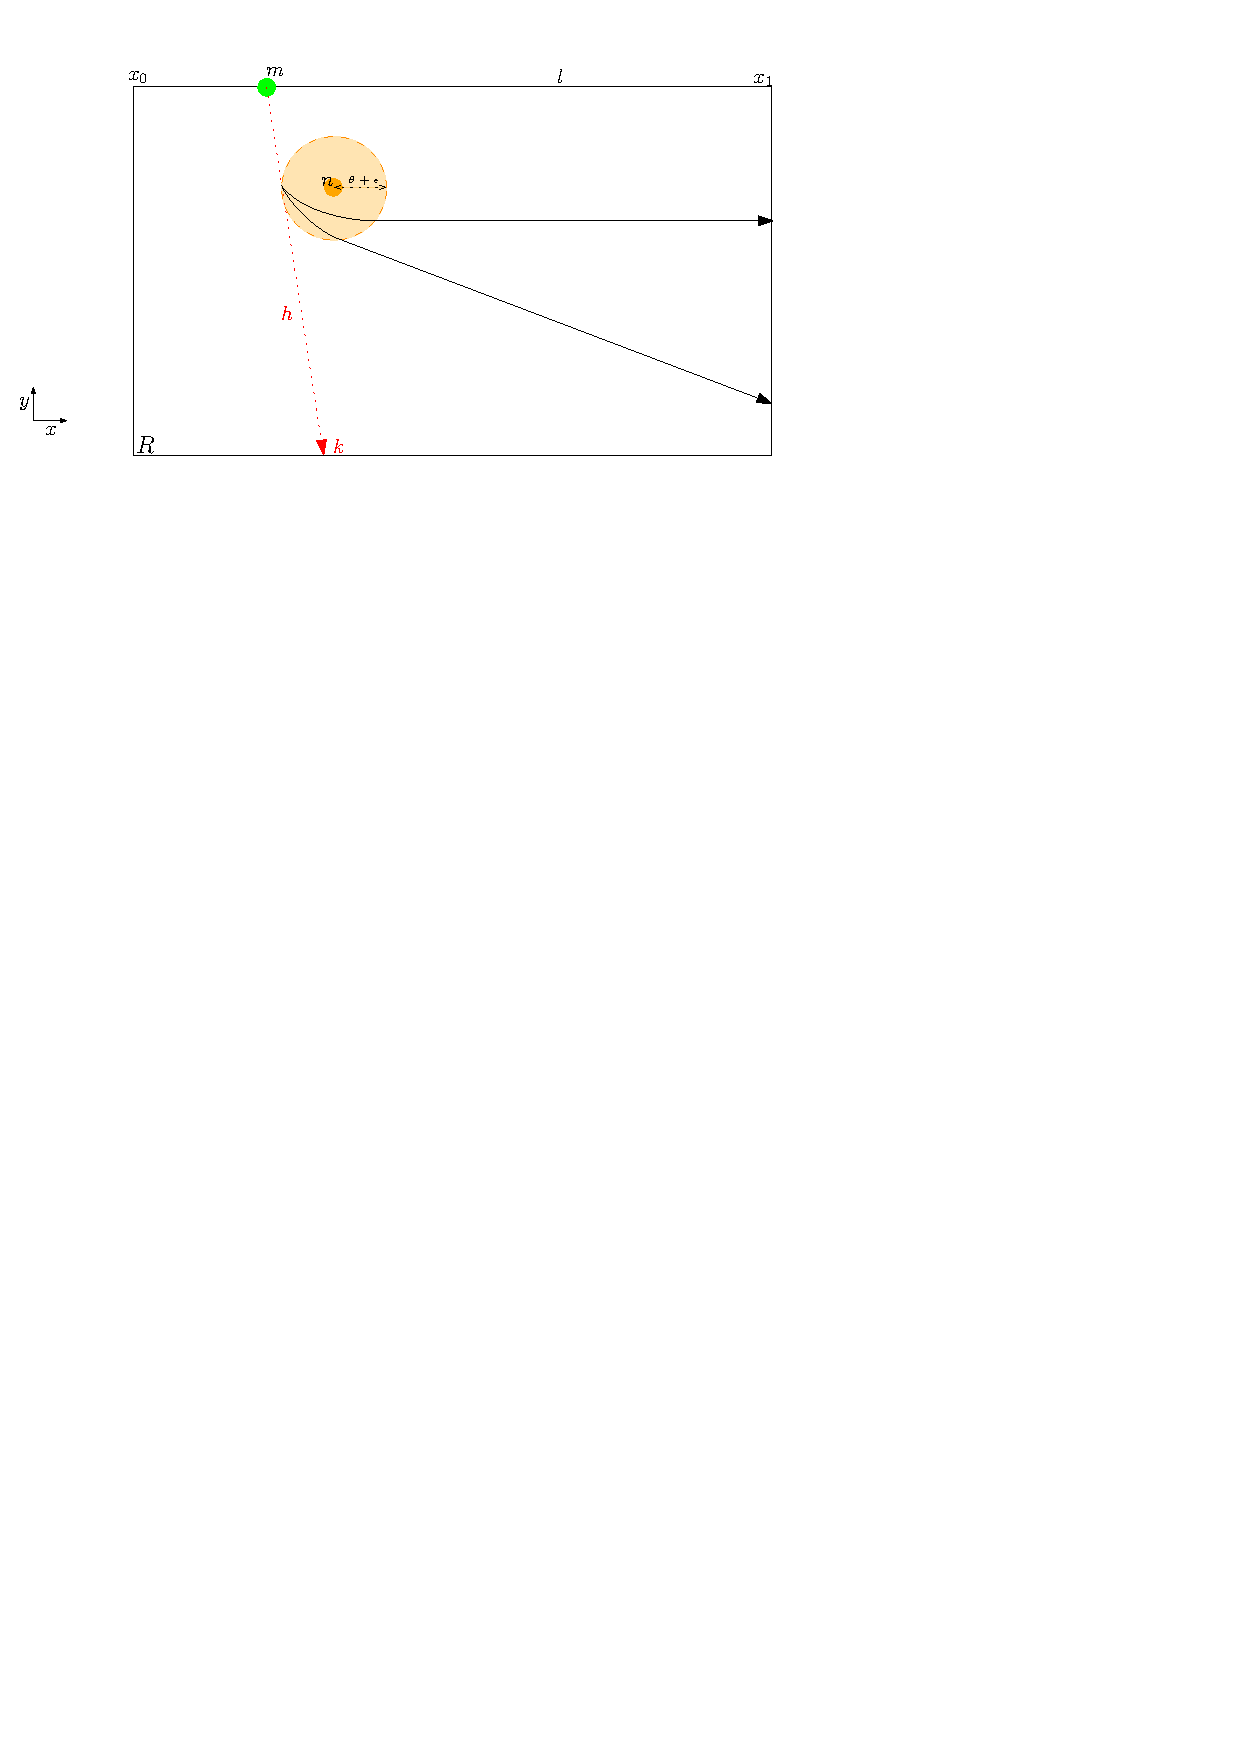
\includegraphics{figures/tunnel_v2.pdf}
    \caption{Construction as used in the proof of Lemma \ref{lemma:tunnel}. The horizontal top edge represents $l$, bounded by $x$-positions $x_0$ and $x_1$. $m$ is the Marble, depicted at the position where it intersects the rectangle $R$ first. The red line represents the path of $m$ if there would be no Node in $R$. The orange point is the node $n$, and the radius of its threshold function has been drawn in transparent orange. Note that $n$ is $\theta$-distance away from $h$, horizontally, hence the radius of the attraction will overlap a little with $h$, which ensures that the movement of $m$ can be influenced by $n$. The black lines represent possible paths trough $R$ of $m$ for two different mass-values of $n$.}
    \label{fig:tunnel}
\end{figure}

\subsection{Bit register}
\nenwin can simulate a single-bit register (i.e. an off-on memory cell).
We present an architecture, for which we can prove the following properties:
\begin{enumerate}
    \item It is possible to read the 0 state
    \item It is possible to read the 1 state
    \item It is possible to set the bit to 0
    \item It is possible to set the bit to 1
\end{enumerate}
The register will be operated by sending a Marble to one of 3 (there is one for reading, one for writing and one for erasing the bit) MarbleEmitterNodes at the edge of the bit. The output will result in a Marble occurring at one of two specific locations that depend on the bit state. This Marble could from there be redirected, or be consumed by a MarbleEaterNode. In the provided architecture the '0-reader' and the '1-reader' are MarbleEaterNodes used at these locations, but for different purposes different elements could be placed here.

\subsubsection{Architecture}
We define the bit architecture $\B$, implemented in $\mathbb{R}^3$ as follows:
\begin{itemize}
    \item Let $P$ be a two-dimensional hyperplane in $\mathbb{R}^3$.
    \item At a specific position in $P$, we create the center of the bit (the 'bit-position'): in the '1' state, this position is occupied by a specific 'bit-Marble', but empty in the '0' state.
    \item A 'bit-emitter' MarbleEmitterNode is placed along the line $l$, which runs though the bit position orthogonal to $P$. We give this MarbleEmitterNode a radius such that the edge of the radius is an infinitesimal distance from the bit position. The Marble that it can emit is the bit-Marble at the bit position.
    \item A 'signal-emitter' MarbleEmitterNode, that is placed at a distance from the bit position in $P$, with a radius sufficiently small not to contain the bit position. The threshold distance is also smaller than the distance from this signal-emitter to the bit-position.
    \item A 'signal-Marble' that can be emitted by the signal-emitter. This Marble has a positive velocity in the direction from the signal-emitter toward the bit-emitter, and is used to pass an external 'write'-signal received by the signal-emitter to the bit-emitter. It has the same mass as the bit-Marble.
    \item Let $\varepsilon \in \mathbb{R}$ be a small yet finite positive number.
    \item A 'read-emitter' MarbleEmitterNode, that is like the signal-emitter also placed in $P$ with a radius and a threshold sufficiently small not to interfere with the bit position. However, it is placed on a different position than the signal-emitter. 
    \item A '0-reader' MarbleEaterNode that is placed in $P$ on the opposite side of the bit position as the read-emitter, but such that the line between the 0-reader and the read-emitter is a distance $\varepsilon$ from the bit position. The radius of this Node can be infinitesimally small, and the threshold distance of its attraction is set to 0.
    \item A 'read-Marble' that can be emitted by the read-emitter, that has an opposite side as the bit-Marble (and hence is repelled by the bit), and a Marble-stiffness of 0. It has a velocity vector in the direction from the read-emitter towards the 0-reader.
    \item A '1-reader' MarbleEaterNode, that is placed in $P$ at an equal distance from the bit-position as the '0-reader', but located such that it will catch the read-Marble if it is repelled by the bit-Marble: it will be proven below that this is not the same location as that of the 0-reader. The radius and the threshold distance have the same values as in the 0-reader.
    \item An 'eraser-emitter' MarbleEmitterNode, similar to the signal-emitter, but at a different position. 
    \item A 'garbage-collector' MarbleEaterNode with similar properties as the 0-reader and the 1-reader, but located exactly on the line running from the eraser-emitter to the bit-position, on the opposite side of the bit-position as the eraser-emitter (this is also in $P$). This Node solely functions to delete Marbles.
    \item An 'eraser-Marble' that can be emitted from the eraser-emitter, with a velocity in the direction from the eraser-emitter towards the bit-position (and hence also towards the garbage-collector). The mass of this eraser-Marble will have the opposite sign as the bit-Marble, and it will have a Node- and Marble-stiffness of 1. The gravity threshold distance of this eraser-Marble is nonzero.
\end{itemize}

The Nodes defined above can all be placed in $\mathbb{R}^3$, on different positions while satisfying their description. All Nodes and Marbles defined above, except the bit-emitter, are placed in $P$ \footnote{It is also possible to place the bit-emitter in $P$, but this would lead to more complex proofs as we need to ensure that it will not interfere with any Marble moving though $P$.}. 

Note that $\B$ should be placed in a region of $\mathbb{R}^3$ where no external forces (except for the Marble that activates reading/writing/erasing) apply, and that when using the threshold gravity function \ref{eq:tresholdgrav}.

The particles of $\B$ and their important properties have been summarized in Table \ref{table:bit}.

\begin{table}[h]
    \begin{tabular}{l|l|l|l|l}
    \textbf{Particle} & \textbf{Type} & \textbf{Mass sign} & \textbf{Marble-stiffness} & \textbf{Marble-attraction} \\ \hline
    bit-Marble        & Marble            & - & 0 & 1 \\
    bit-emitter       & MarbleEmitterNode & 0 &   &   \\
    signal-emitter    & MarbleEmitterNode & 0 &   &   \\
    signal-Marble     & Marble            & - &   &   \\
    read-emitter      & MarbleEmitterNode & 0 &   &   \\
    0-reader          & MarbleEaterNode   & + &   &   \\
    reader-Marble     & Marble            & + & 0 & 0 \\
    1-reader          & MarbleEaterNode   & + &   &   \\
    eraser-emitter    & MarbleEmitterNode & 0 &   &   \\
    garbage-collector & MarbleEaterNode   & 0 &   &   \\
    eraser-Marble     & Marble            & + & 1 & 1
    \end{tabular}
    \caption{Summary of the particles in $\B$, with their most important attributes. 
    Irrelevant values have been omitted: the bit can be made to work for multiple values of these variables. For the mass only the sign and not the magnitude has been recorded, except where the mass is 0. Note that it may not be strictly required to make those particles mass-less, but it simplifies the proof.}
    \label{table:bit}
\end{table}


\begin{figure}
    \centering
    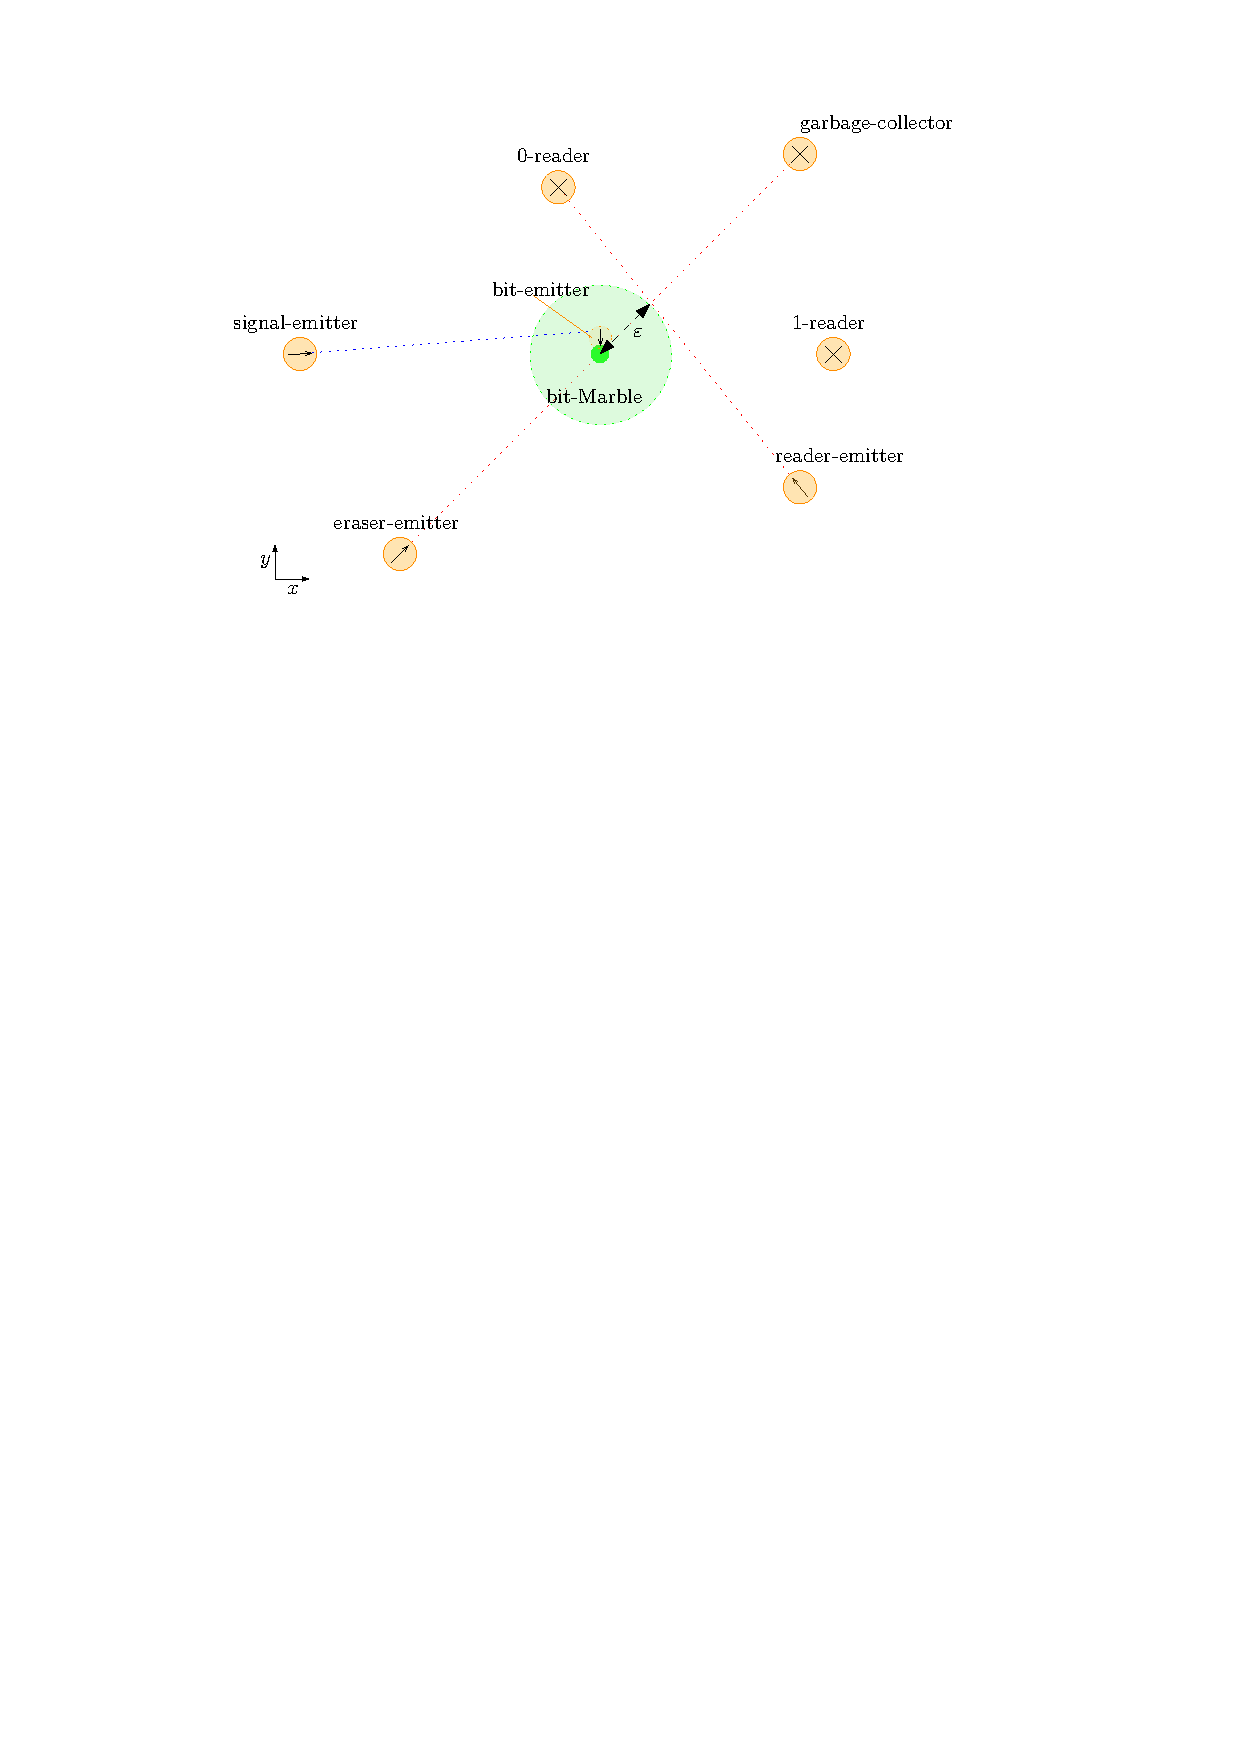
\includegraphics{figures/bit_base.pdf}
    \caption{A visualization of the bit-register architecture $\B$, as projected on a 2-dimensional image. Nodes are drawn in orange, and MarbleEmitterNodes bear an arrow that point in the direction of the velocity of the Marble they can emit. The Bit-Marble is drawn in green, with the threshold-gravity-radius drawn in light-green. Note that the distances and sizes are not necessary to scale.}
    \label{fig:bit_architecture}
\end{figure}

Let $\gamma \subseteq \mathbb{R}^3$ denote the smallest continuous cuboid region in $\mathbb{R}^3$ in which $\B$ has influence (i.e. all particles of $\B$ and all their attraction fields are contained in $\gamma$). 

\begin{lemma}[Reading state 0]
    An external Marble can trigger architecture $\B$ to increase the output of the 0-reader by 1 if the bit register is in the 0-state. After this operation, $\B$ will be in the same state as it started except for the value of the 0-reader.
    \label{lemma:0-reader}
\end{lemma}
\begin{proof}
    Consider an external Marble that enters $\gamma$ at the facet of $\gamma$ that is closest to the reader-emitter, and let this Marble have velocity that moves it in a straight line to the reader-emitter. If this Marble has the correct mass, then the reader-emitter will emit a reader-Marble. This reader-Marble has an initial velocity in the direction of the 0-reader, by design of $\B$. Since there is no bit-Marble to alter its course of motion (since the bit is in state 0) nor any other attraction along its way, it will arrive at the 0-reader. 
    
    Note that the reader-Marble cannot intersect the radius of the bit-emitter, since the bit-emitter does not intersect the plane $P$, in which the reader-Marble remains its entire existence (it moves along the line from the reader-emitter to the 0-reader. These two Nodes are in $P$, and therefore this entire line is in $P$).
    
    Clearly, no particles that existed before the external Marble entered $\gamma$ have been changed during this operation, except for the state of the 0-reader.
\end{proof}

\begin{lemma}[Reading state 1]
     There exists a location for the 1-reader, a value for $\varepsilon$, a mass value and a gravity threshold value for the bit-Marble, such that an external Marble can trigger architecture $\B$ to increase the output of the 1-reader by 1, if the bit register is in the 1-state. After this operation, $\B$ will be in the same state as it started except for the value of the 1-reader.
     \label{lemma:1-reader}
\end{lemma}
\begin{proof}
    As in Lemma \ref{lemma:0-reader}, an external Marble can cause the reader-emitter to emit a reader-Marble. Since the state of the bit is 1, there is a bit-Marble at the bit-position. Now we can adjust $\varepsilon$ the threshold of the bit-Marble's gravity such that the path of the reader-Marble will intersect the attraction field of the bit-Marble at its boundary. Let $p$ the point where this boundary and the line between the reader-emitter and the 0-reader (which define $\varepsilon$) intersect. 
    
    The direction of movement the reader-Marble will not be altered form its starting velocity until it reaches point $p$. Since the mass of the bit-Marble is by construction of the opposite sign as that of the reader-Marble, and since the reader-Marble does not attract Marbles but is attracted by them (by construction), only the acceleration of the reader-Marble will be affected. The reader-Marble will be accelerated in the same direction as the line segment between the bit-position and $p$, and this direction is orthogonal to the direction reader-Marbles initial velocity. 
    
    Since the reader-Marble intersects only shortly this acceleration is present only one instant of time. However, if the mass of the bit-Marble is of sufficient magnitude, it will change the direction of the velocity of the reader-Marble significantly. The new direction of this velocity is not the opposite of the original direction, as the acceleration was orthogonal to the original velocity of the reader-Marble. Hence the reader-Marble will not arrive at the reader-emitter (which requires the opposite direction as the original velocity of the reader-Marble had) nor the 0-reader (which requires the original direction). 
    
    Note that the reader-Marble cannot intersect the radius of the bit-emitter, since the bit-emitter does not intersect the plane $P$, in which the reader-Marble remains its entire existence.
    (as in Lemma \ref{lemma:0-reader}, the initial path of the reader-Marble is in $P$. Since $p$ is on the line between the reader-emitter and the 0-reader, $p$ is in $P$ as well. Now since the bit-position is also in $P$, the acceleration vector is also in $P$. The resulting velocity of the reader-Marble is a linear combination of its prior velocity and the acceleration, which are both vectors in $P$, hence the reader-Marble remains in $P$.)
    
    The 1-reader can be positioned along the line from the reader-Marble in the new direction of the Marble's velocity, and then the reader-Marble will eventually be consumed by the 1-reader.
\end{proof}

\begin{lemma}[Writing bit]
    An external Marble can trigger architecture $\B$ when in state 0 (no bit-Marble present) to enter state 1 (with a bit-Marble present), without any other particle in $\B$ being affected after completion.
    \label{lemma:writing}
\end{lemma}
\begin{proof}
    Let the external Marble enter $\gamma$ in the point closest point of the closest facet of $\gamma$ to the signal-emitter, with a velocity the direction of the line from that point to the signal-emitter. Then this Marble will be consumed by the signal-emitter, and if it of sufficient mass it will trigger the signal-emitter once to emit a signal-Marble.
    
    The signal-Marble is configured (by construction of $\B$ to have a velocity in the direction of the signal-emitter towards the bit-emitter, and since it is not attracted by Marbles or Nodes, nor does any Eater- or EmitterNode block its path, it will eventually be consumed by the bit-emitter. Consequently, the bit-emitter creates a single bit-Marble.
\end{proof}

\begin{lemma}[Erasing bit]
    An external Marble can trigger architecture $\B$ when in state 1 (a bit-Marble present) to enter state 1 (no bit-Marble present), without any other particle in $\B$ being affected after completion, except for the mass stored in the garbage-collector.
    \label{lemma:erasing}
\end{lemma}
\begin{proof}
    Let the external Marble enter $\gamma$ in the closest point of the closest facet to the eraser-emitter, with a velocity in the direction of the line from this point towards the eraser-emitter. The Marble will be consumed by the signal-emitter, and if the external Marble had enough mass, an eraser-Marble will be emitted in the direction of the bit position. Note that the eraser-Marble has both a Node- and Marble-stiffness of 1, hence no attraction force will affect its acceleration. Hence it will travel in a straight line with constant velocity.
    
    The eraser-Marble has a Marble-stiffness of 1, and since the bit-Marble has a Marble-stiffness of 0, the bit-Marble's motion will be affected when the eraser-Marble nears the bit-Marble. Since the mass of the eraser-Marble is of the opposite sign as that of the bit-Marble, it will repel the bit-Marble, which will be accelerated in the same direction as the eraser-Marble is moving. Now we can adjust the masses of the bit-Marble and the eraser-Marble such that the repellent force is strong enough the accelerate the bit-Marble to the same or a higher velocity as the eraser-Marble before the eraser-Marble reaches the bit-position: this will guarantee that the eraser-Marble will not 'take-over' the bit-Marble and repel it in the other direction.
    
    Now both Marbles will travel in the direction of the line from the eraser-emitter to the bit-position. By construction of $\B$, the garbage-collector is also on this line and on the other side of the bit-position as the eraser-emitter. Therefore both Marbles will eventually enter the radius of the garbage-collector and be absorbed.
\end{proof}

We can summarize the results of Lemma \ref{lemma:0-reader}, \ref{lemma:1-reader}, \ref{lemma:writing} and \ref{lemma:erasing} in the following theorem:

\begin{theorem}[Bit register]
    There exist settings for the parameters of $\B$, and an external Marble $m$ outside of $\gamma$, such that by moving $m$ with the right value of $m.vel$, $m.pos$ and $m.mass$ into $\gamma$:
    \begin{enumerate}
        \item $m$ can trigger the reading of the bit. That is, after sufficient time, if there is a bit-Marble present, the 1-reader's number-of-Marbles-consumed count will increase by 1. If there no bit-Marble present, after sufficient time, the count of the 0-reader will increase by 1. When this count increases, the collection of particles in $\gamma$ and their states are identical to the situation before $m$ entered $\gamma$.
        \item $m$ can cause the creation of a bit-Marble in $\B$ without affecting the state of other particles in $\B$.
        \item $m$ can cause the removal of a bit-Marble in $\B$, when present, without affecting the state of other particles in $\B$ except for the Marbles consumed by the garbage-collector.
        \item Furthermore, $\B$ does not directly affect particles outside $\gamma$.
    \end{enumerate}
\end{theorem}
\begin{proof}
    \begin{enumerate}
        \item Follows from Lemma \ref{lemma:0-reader} and Lemma \ref{lemma:1-reader}.
        \item Follows from Lemma \ref{lemma:writing}.
        \item Follows from Lemma \ref{lemma:erasing}.
        \item The particles in $\B$ are constructed around a finite distance from the bit-position in $\mathbb{R}^3$, use finite radii and are using the threshold gravity as attraction function with a finite threshold. Hence in each direction from the bit-position, there is a distance that surpasses the influence of attraction functions, radii and positions of particles. By construction of $\gamma$, the minimum value of this distance either defines a facet of $\gamma$ or is interior to $\gamma$. Hence outside $\gamma$, $\B$ cannot affect any particle directly.
    \end{enumerate}
\end{proof}

\subsection{Clock and divider}
Implementing a clock in \textsc{Nenwin} is trivial: a MarbleEmitterNode with a large amount of \texttt{stored\_mass} (e.g. a value of $\infty$) and a positively-valued delay will already periodically emit a Marble. Since Marbles are used to represent signals, this suffices to implement a periodical signal-creating device. However, the signal needs to reach multiple components after a sufficiently large delay, and a single Marble can be absorbed only once. Multiple clocks could be used, but a solution that reduces the amount of clocks needed is to use 'splitters':
\begin{lemma}
    Given a finite region $R \subset \mathbb{R}^x$ ($x \geq 2$) in a \textsc{Nenwin} architecture with no external forces, it is possible to construct an architecture in $R$ such that when a Marble $m$ with mass $\alpha$ enters $R$ at a designated point $q$ at $t_0$, that this causes any fixed amount $n \geq 0$ Marbles to be emitted from $R$ with velocities in different directions, at a time $t_0 < t_1 < \infty$. This architecture in $R$ will not emit Marbles or exerts forces outside $R$ otherwise.
    \label{lemma:splitter}
\end{lemma}
\begin{proof}
    The case when $n = 0$ is trivial, a single MarbleEaterNode positioned in $R$ with 0 Marble- and Node-attraction and a radius that intersects $q$.
    
    For $n \geq 1$, consider the following architecture (where all particles have a Marble- and Node-stiffness of 1 unless denoted otherwise) (see also Fig. \ref{fig:splitter}):
    \begin{itemize}
        \item Let $P$ be a rectangle on a plane though $R$ with maximal surface area.
        \item A 'signal-emitter': a MarbleEmitterNode, positioned such in $P$ with such a radius that the border of the radius intersects the border of $R$. It has a delay of $\delta$.
        \item Let $l$ be the ray parallel to $P$ that starts in the signal-emitter and that intersects the center of $P$.
        \item A 'signal-Marble': the Marble that can be emitted by the signal-emitter. Let it have a mass of $\alpha$ and a velocity direction parallel to the $l$ (towards the centre of $P$) and a velocity magnitude of $v_{signal}$. 
        \item Two 'locker-Nodes': two Nodes with the same negative mass, placed in $P$, both on a line $l'$ in $P$ orthogonal to $l$ that also intersects the center of $P$, each at a different side of $l$, each at an equal distance from $l$. Their threshold distance of their attraction functions have the same positive value. Let these Nodes have a Marble-attraction of 0 and a Node-attraction of 1.
        \item A 'moving-emitter': a MarbleEmitterNode initially placed with a specific positive mass and a specific velocity $v_{Node}$ at a specific point $p'$ on $l'$ where the distance to the clostest locker-Node is $d + \varepsilon$, such that it will be deaccelerated by locker-Node untill it halts on a point $p$ at a distance $d$ from this locker-Node, and will reverse its direction when it is a distance $d$ from that locker-Node: hence $p'$ is an extreme point of the harmonic motion this moving-emitter will show. Let $\delta$ be the period of the harmonic motion. Let the moving-emitter have a delay of $\frac{delta}{2\cdot n}$. Let this Node be the only Node in $R$ with a Marble- and Node-stiffness both of 0.
        \item Let $v_{signal}$ equal $\frac{\frac{\varepsilon}{v_{Node}}}{z}$  where $z$ is the smallest component parallel to $l$ of the distance form the point where the signal-Marble is emitted to the border of the radius of the moving-emitter (which equals the distance from the point where the signal-Marble is created to the closest border of the signal-emitter when the latter is in the point $p$).
        \item $n$ 'output-emitters' named $O_1, O_2, \dots, O_n$, placed in $P$ on the opposite side of $l'$ as the signal-emitter is, such that at a time $t_0 + i \cdot \frac{\delta}{2 \cdot n} \mod \delta$ the moving-emitter is in a position where a line-segment $k_i$ exists in $P$ that is parallel to $l$ and intersects both the moving-emitter and $O_i$ for $1 \leq i \leq n$, and such that the position and radius have that the border of their radius intersect the border of $R$. 
        \item Let the 'split-Marbles' be the Marbles emitted by the moving-emitter with a mass of $\frac{\alpha}{2}$ and a velocity parallel to $l$ (away from the center of $P$).
    \end{itemize}
    Note that the distance between each line segment $k_i$ and $k_j$, $1 \leq i < j \leq n$ is not necessarily equal as the moving-emitter does not have a constant velocity and hence does not travel a fixed amount of distance in the same time span.
    
    Now if $m$ is consumed by the signal-emitter at time $t = t_0$, it will emit a signal-Marble. By construction of the moving-emitter, it will be at point $p$ at time $t = t_1 = t_0 + \frac{\varepsilon}{v_{Node}}$. But by construction, this is also the time required by the signal-Marble to travel to the point where it would be consumed by the moving-emitter if it were at point $p$. Since the moving-emitter is at point $p$, it will consume the Marble. By definition of point $p$, this is the point where the direction of the velocity of the moving emitter reverses in direction. So at time $t = t_1 + \frac{delta}{2\cdot n}$, by construction, the moving-emitter will be positioned on $k_1$. Since its first delay has been satisfied, it will emit the first split-Marble, which is created in such a position where it will move in a direct line to $O_1$. Now the \texttt{stored\_mass} of the moving-emitter is $\alpha - \frac{\alpha}{n}$. The same process is repeated for $O_2$, $O_3$, \dots, $O_n$. Let $\hat{p}$ the point that is the image of $p$ when mirroring $p$ in $l$ on $P$. Because of the harmonic motion, the moving-emitter will reverse its direction again at point $\hat{p}$, but at this point its \texttt{stored\_mass} is 0. Hence on the 'return trip' to $p$ it will not emit any Marble. Now each of the output-emitters $O_1$, $O_2$, \dots, $O_n$ has received exactly one split-Marble. Since each of the output-emitters intersects the boundary of $R$, each can create an output Marble outside $R$ with a mass of $\frac{\alpha}{n}$, each in a different direction.
    
    At time $t = \delta$, the moving-emitter is at point $p'$ again with a \texttt{stored\_mass} of 0, and if the velocity of the split-Marbles is large enough and the delay of the output-Marbles is small enough, all particles in $R$ will be in the exact same state as at $t_0$.
    
    It remains to prove the harmonic motion of the moving-emitter. Note that if the threshold-distance of the locker-Nodes is at least as far as the distance to the other locker-Node, that the situation is equivalent to the physical model of simple harmonic motion under Newton's model of gravity \cite{principia}. It is beyond the scope of this report to prove simple harmonic motion, but the reader is referred to, for example, \cite{uni_physics}.
\end{proof}
Note that the NAND-gate requires both positively and negatively massed Marbles as 'power' from the clock to operate. This can be implemented by using two synchronized MarbleEmitterNodes, one which emits positively massed Marbles, and the other negatively massed Marbles.

\begin{figure}[h]
    \centering
    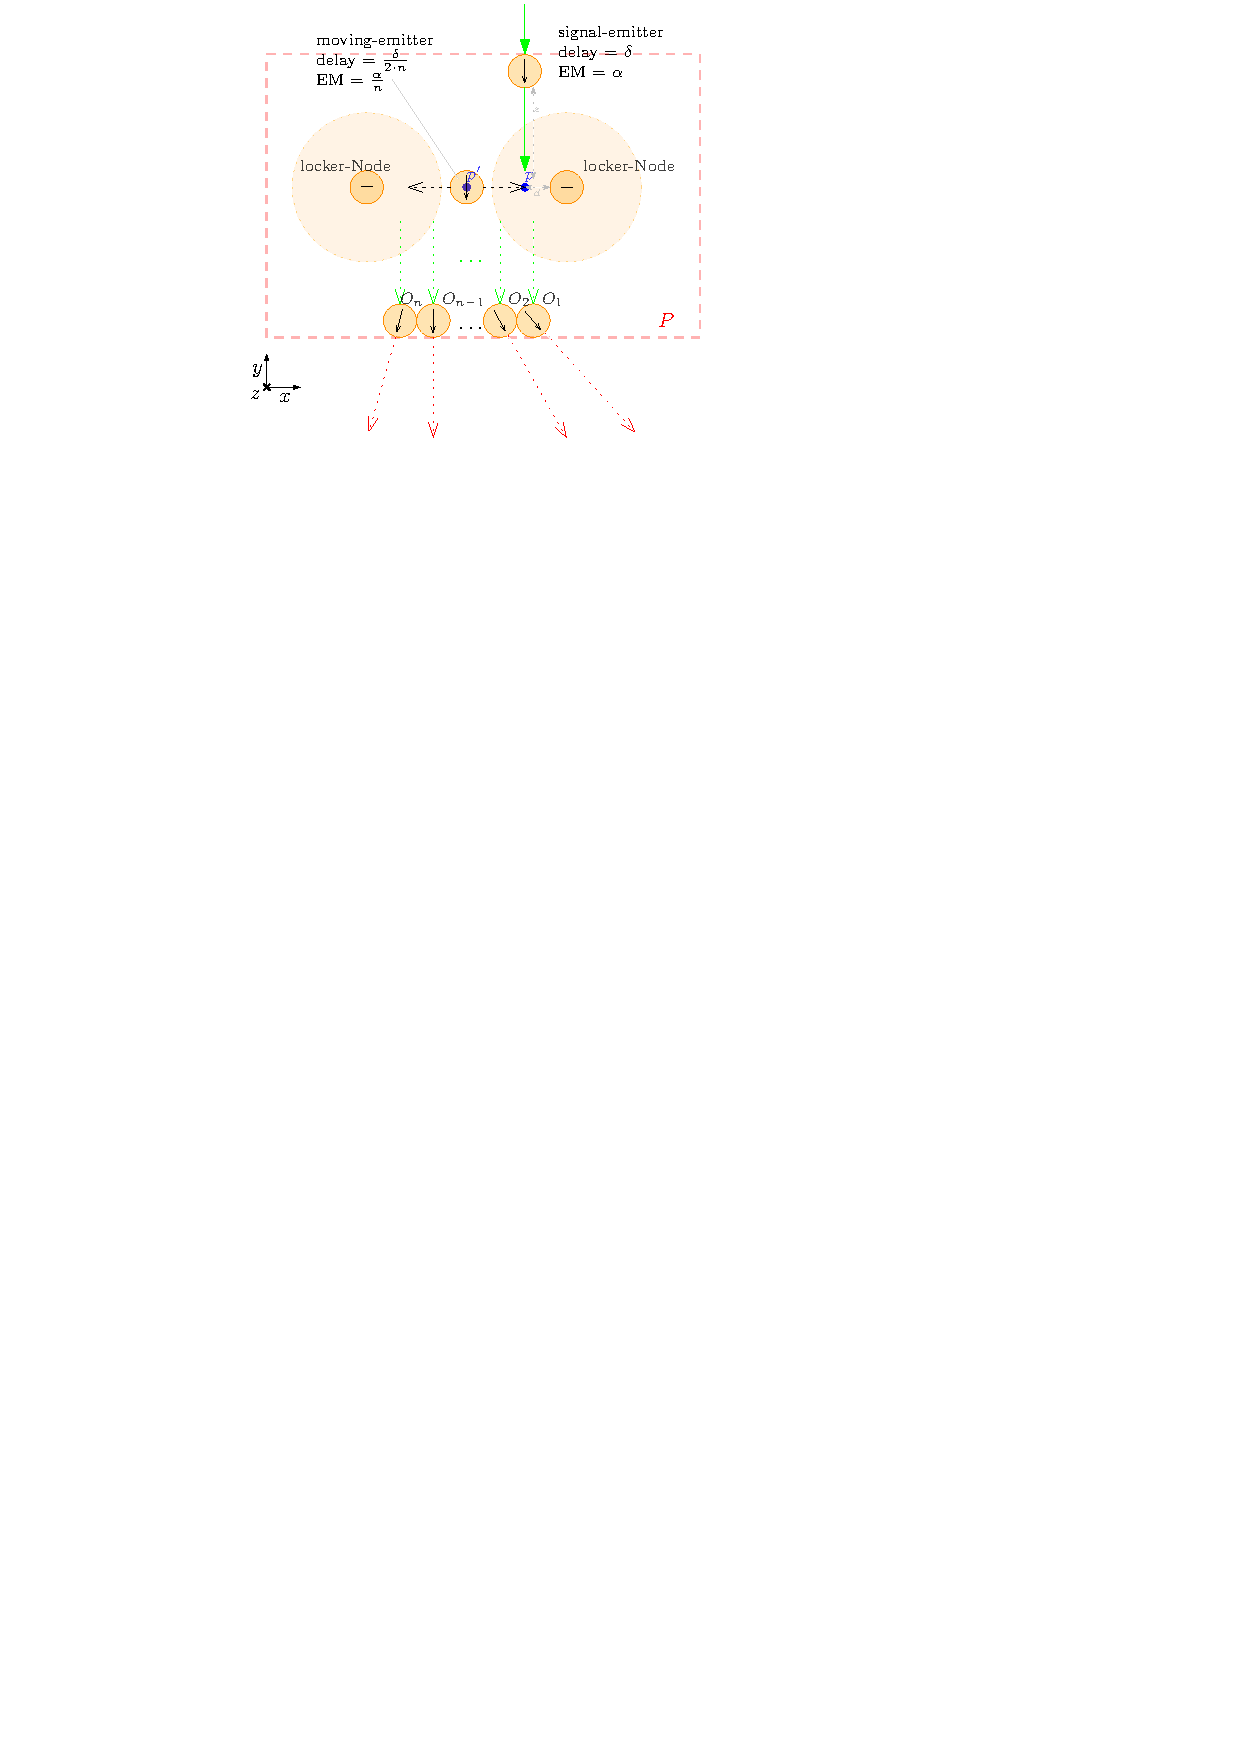
\includegraphics{figures/splitter_v4.pdf}
    \caption{Construction as used in the proof of Lemma \ref{lemma:splitter}. The naming of objects is analogous with the proof. The black dotted arrows denote the directions of velocity of the moving-emitter, the red dotted arrows denote possible directions of velocity of the output Marbles, the green dotted arrows denote the last segment of the movement of the split-Marbles that are released by the moving-emitter, and the continuous green arrows denote the movement of the input-Marble and the signal-Marble.}
    \label{fig:splitter}
\end{figure}



\subsection{Section conclusion}
It is beyond the scope of this report to describe a complete implementation of a CPU in \textsc{Nenwin}, but sufficient important components have been described to abstract from the implementations of components, and reason on the (sequential) logical circuit level of abstraction. How to design a CPU with such circuits has been described in many sources, such as \cite{comp_architecture} and \cite{comp_org_design}.

\clearpage